% Section: Client Usage
This section contains all information needed by end users to successfully use
the \textan{} client application. For instructions to actual run the client
see Section \ref{sssec:StartClient}. \comment{Ondrej}{I do not understand what
will be there, why chapter 2 and not sooner?}

\subsection{First Run}

On the first run of \textan{} client, users are prompted to enter their username
(see Figure \ref{fig:Login}, which is used by the system to identify the users.
The login name is stored in settings and the login dialog is not shown again
in following runs. The name can be changed in settings (see Section
\ref{ssec:Settings}). A valid name is required, ie. not empty and not whitespace
characters only. If users enter invalid login, a warning is displayed and they
may enter other login or the application quits.

\begin{figure}[!htb]
        \centering
        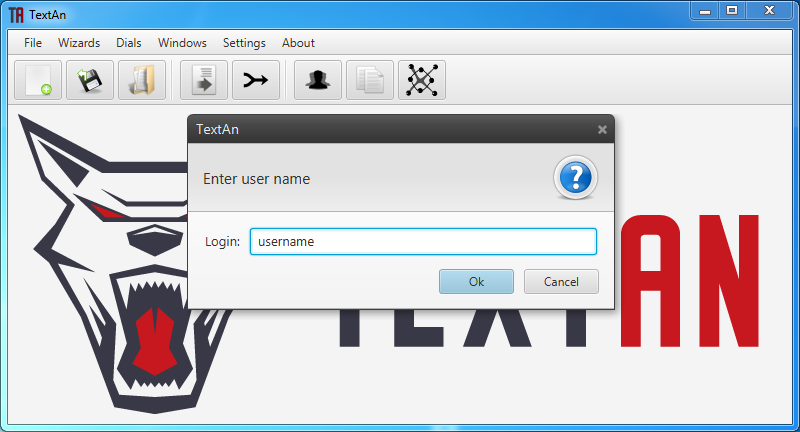
\includegraphics[width=\textwidth]{Images/login}
        \caption{Login prompt on first run.}
        \label{fig:Login}
\end{figure}

\subsection{Working Space}

The \textan{} client's application working space is very simple and intuitive.
The main window (see Figure \ref{fig:MainWindow}) contains the main menubar with
all commands needed to control the application. There is also a toolbar with
icons for mostly used commands to speed up the access. Hover over the
toolbar icons to see the corresponding action names.

\begin{figure}[!htb]
        \centering
        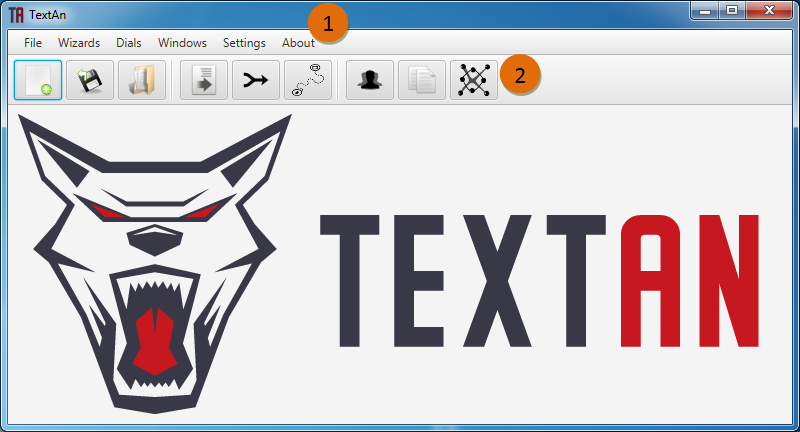
\includegraphics[width=\textwidth]{Images/main}
        \caption{Main window controls. 1) Main menubar, 2) Toolbar.}
        \label{fig:MainWindow}
\end{figure}

The File menu contains items to create new report, import report from external
file and load report whose processing was not finished, but was saved to continue
later. For more information about report processing, see Section \ref{ssec:ProcessReport}.

The Wizards menu contains items starting wizards to guide the users in more
complicated tasks, like processing report (see Section \ref{ssec:ProcessReport})
and joining objects (see Section \ref{ssec:JoinObjects}).

The Dials menu contains items to display objects, documents and relations
stored in the database (see Section \ref{ssec:ViewDatabase}).

The Windows menu contains the list of currently displayed application windows
to easily bring certain window to front.

The Settings menu contains items to customize \textan{} client appearance and
behavior. For more information, see Section \ref{ssec:Settings}. It also
contains shortcut to reset the position and size of the main window.

\subsection{Settings}
\label{ssec:Settings}

This section describes options available in individual items contained in the
main menu Settings. All these settings are safe to change by end user. For
more advance options, please see Sections \ref{sssec:BasicConf} and
\ref{ssec:ClientSettings}.

\subsubsection{General Settings}
\label{sssec:GeneralSettings}

The General Settings window (see Figure \ref{fig:GeneralSettings}) contains
controls for changing the behavior and appearance of the application.

\begin{figure}[!htb]
        \centering
        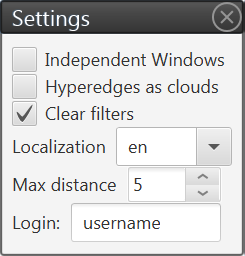
\includegraphics{Images/general}
        \caption{General Settings Window}
        \label{fig:GeneralSettings}
\end{figure}

\paragraph{Independent Windows} If this control is checked, the application
secondary windows will not be embedded into the main window, but separate
independent system windows will be used.

\paragraph{Hyperedges as clouds} This control affects the rendering of
hyperedges\footnote{Hyperedge is an edge in a hypergraph which is a
generalization of term graph. The difference is that edges in hypergraphs can
connect any number of nodes, whereas in graph they always connect two nodes.}
in graphs (see Figure \ref{fig:Hypergraphs}). The default rendering transforms
hypergraphs to graphs by adding auxiliary nodes of square shape representing
the relation. If this control is checked, the edges are rendered by graph
background.

\begin{figure}[!htb]
        \centering
        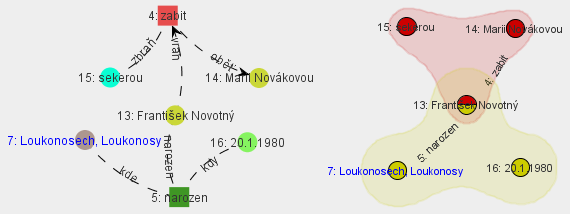
\includegraphics[width=\textwidth]{Images/hypergraphs}
        \caption{Graph rendering differences. Default on the left.}
        \label{fig:Hypergraphs}
\end{figure}

\paragraph{Clear Filters} If this control is checked, the filter fields
displayed during report processing will be cleared when shown again.

\paragraph{Localization} This control determines the language of the \textan{}
client. The Czech and English localizations are currently supported. The
default language is English. Changing localization takes effect after
restarting the application.

\paragraph{Max Distance} This control affects the default maximal length of the
path between any node and the graph central node. Nodes beyond this limit are
not displayed.

\paragraph{Login} This control enables users to change their username. Changing
login takes effect after restarting the application.

\subsubsection{Colors}
The Colors settings window (see Figure \ref{fig:Colors}) contains two lists -
one for object types and one for relation types. They contain all types found
in the database and enable users to easily customize their color displayed in
graphs views and report processing windows by clicking corresponding color
pickers.

\begin{figure}[!htb]
        \centering
        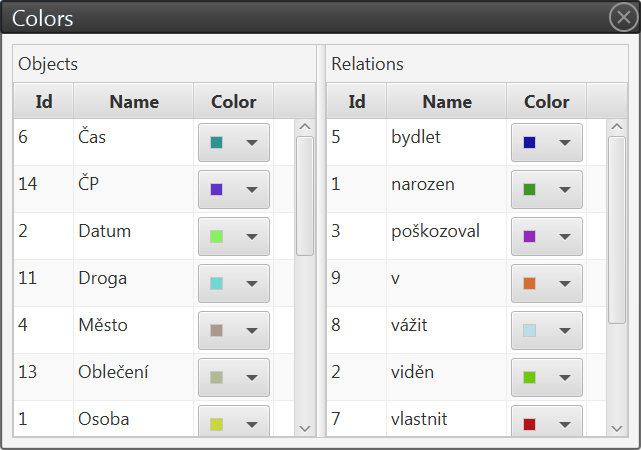
\includegraphics[width=\textwidth]{Images/colors}
        \caption{Colors settings window.}
        \label{fig:Colors}
\end{figure}

\subsection{Report Processing}
\label{ssec:ProcessReport}

The wizard for report processing is accessible from the main menu. It guides
users in complicated procedure of processing a report. The procedure is divided
into several steps described in this section (see figure \ref{fig:Pipeline}).
Users can return to previous steps, but if any changes are done, the progress
in following steps is lost.

\begin{figure}[!htb]
        \centering
        
\includegraphics[height=16cm,keepaspectratio]{Images/pipeline}
        \caption{Schema of report processing.}
        \label{fig:Pipeline}
\end{figure}

In Edit Report step and later, when the report processing is interrupted,
\textan{} offers to save the unfinished report into a file. The processing can
be resumed by selecting Unfinished Report in Report Source step (see Section
\ref{sssec:ReportSource}). The processing continues in the step where it was
saved.

\subsubsection{Report Source}
\label{sssec:ReportSource}

\begin{figure}[!htb]
        \centering
        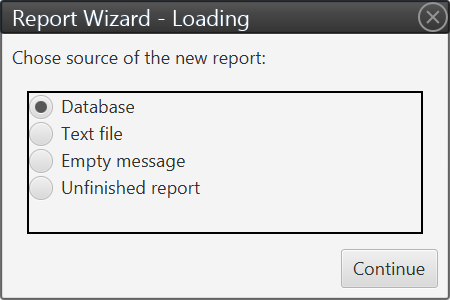
\includegraphics{Images/source}
        \caption{Choosing report source.}
        \label{fig:Source}
\end{figure}

This step (see Figure \ref{fig:Source}) allows users to choose the source of the
report. The following sources are possible:

\paragraph{Database} This option displays (see Figure \ref{fig:Database}) list
of all unprocessed reports stored in the database (for filtering details see
Section \ref{sssec:DocumentList}).
The report cannot be edited, so the wizard then proceeds to Edit Entities step
(see Section \ref{sssec:EditEntities}). \comment[Adam]{Ondrej}{The following is
not completely comprehensible} If the report is edited by someone else
externally while being processed by a local user, a warning message is
displayed. The local user can decide whether the report processing should end or
continue with the current text. In the latter case, the current text overwrites
the one in the database when processed report is saved to the database. It is
also possible to enter Edit Report step and edit it as it will replace stored
text anyway.

\begin{figure}[!htb]
        \centering
        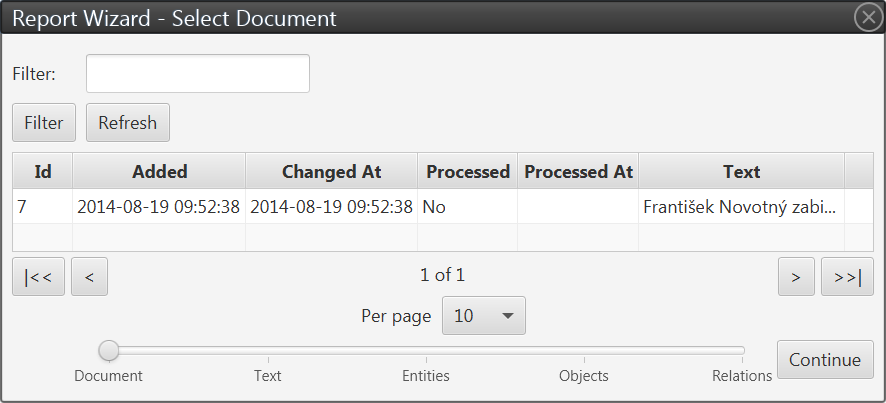
\includegraphics[width=\textwidth]{Images/database}
        \caption{Chosing report from database.}
        \label{fig:Database}
\end{figure}

\paragraph{Text File} This option displays open file dialog for importing
report text from external file. The extracted text is then displayed (see
Figure \ref{fig:TextFile}, so users can chose the proper file encoding. Then
the wizard proceeds to Report Edit step (see Section \ref{sssec:ReportEdit}).

\begin{figure}[!htb]
        \centering
        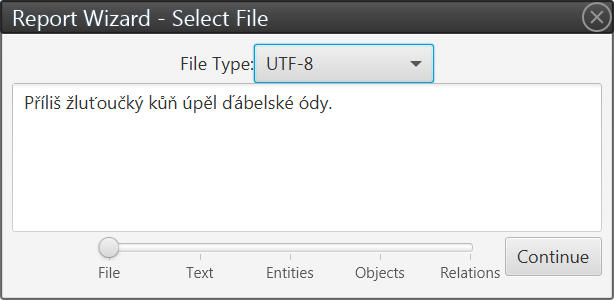
\includegraphics[width=\textwidth]{Images/textfile}
        \caption{Chosing encoding of the file.}
        \label{fig:TextFile}
\end{figure}

\paragraph{Empty Message} This option proceeds directly to Report Edit step
(see Section \ref{sssec:ReportEdit}) with empty report.

\paragraph{Unfinished Report} This option displays open file dialog for
selecting the file with report whose processing has not been finished, but it
was stored to continue later. The wizards then proceeds to step where report
processing has been interrupted.

\subsubsection{Edit Report}
\label{sssec:ReportEdit}

In this step users can edit the text of the report (see Figure
\ref{fig:ReportEdit}. This step is followed by Edit Entities step (see Section
\ref{sssec:EditEntities}).

\begin{figure}[!htb]
        \centering
        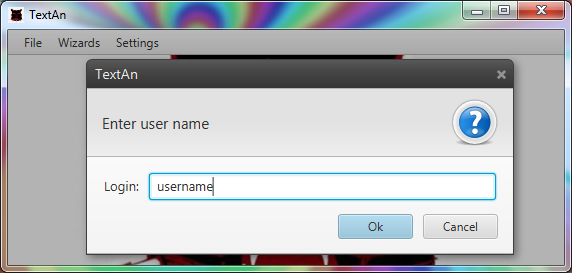
\includegraphics[width=\textwidth]{Images/reportedit}
        \caption{Editing the text of the report.}
        \label{fig:ReportEdit}
\end{figure}

\subsubsection{Edit Entities}
\label{sssec:EditEntities}

Before entering this step the system automatically recognizes named entities
in the report text. Recognized entities are marked by text color. Entities of
the same type have the same color (see Figure \ref{fig:Entities}). Hovering over
entity text will display its type.

Users can correct recognized entities and add new ones by selecting the text
of the entity by mouse and picking the entity type from the context menu.
There is a filter field in the context menu to allow users enter substring of
name of the desired entity type to speed up the selection process. If there are
only one item in the list left, it can be selected by pressing enter too.
Pressing Down key in the filter field transfers focus to the list, so keyboard
keys Up, Down and Enter can be used to select the entity type.

One entity cannot comprise from several separated parts and entities cannot
overlap.

This step is followed by Edit Objects step (see Section
\ref{sssec:EditObjects}).

\begin{figure}[!htb]
        \centering
        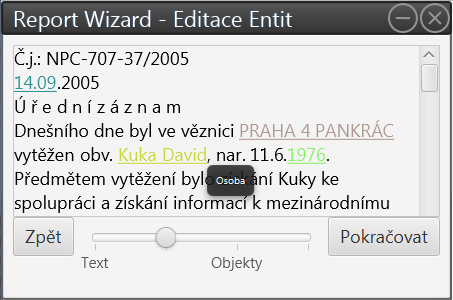
\includegraphics[width=\textwidth]{Images/entities}
        \caption{Editing entities in the report.}
        \label{fig:Entities}
\end{figure}

\subsubsection{Edit Objects}
\label{sssec:EditObjects}

In this step the entities are assigned to real objects (see Figure
\ref{fig:Objects}). The system automatically assigns objects stored in the
database to entities recognized in the database. If no suitable object is
found, the entity is marked with orange background. Hovering over entity
displays its type and assigned object if any.

\begin{figure}[!htb]
        \centering
        
\includegraphics[width=\textwidth]{Images/objects}
        \caption{Editing objects in the report.}
        \label{fig:Objects}
\end{figure}

Right click on objects will display context menu with options to show the graph
of the object or documents containing the object. This is also true for all following steps.

To assign object to entity left click the entity and select suitable object
from the context menu (see Figure \ref{fig:ObjectMenu}) or create entirely new
object.

\begin{figure}[!htb]
        \centering
        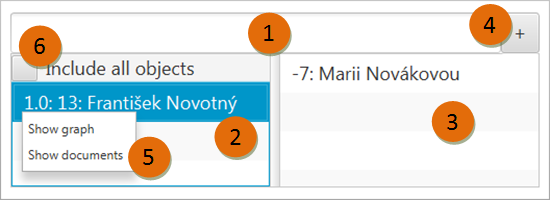
\includegraphics[width=\textwidth]{Images/objectmenu}
        \caption{Menu for selecting object. 1) Filter field, 2) List of
		 recommended objects (with probability of match), if 6) is checked, list
		 of objects of given type from database, 3) List of new objects created
		 during editation of the same type, 4) Button for creating new object,
		 5) Menu for more information about the object.}
        \label{fig:ObjectMenu}
\end{figure}

The report processing cannot continue unless all entities have assigned
objects. This step is then followed by Relation Edit step (see Section
\ref{sssec:EditRelations}).

\subsubsection{Edit Relations}
\label{sssec:EditRelations}

This is the last mandatory step during report processing (see Figure
\ref{fig:Relations}). It consists of marking relationships between objects in
the document.

\begin{figure}[!htb]
        \centering
        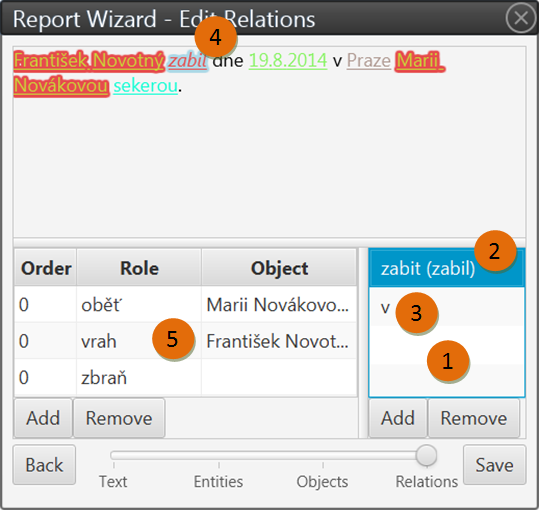
\includegraphics[width=\textwidth]{Images/relations}
        \caption{Editing relations in the report. 1) Relation list, 2) Relation
		 with anchor, currently selected, 3) Relation without anchor, 4) Highlighted
		 relation anchor, note highlighted objects too, 5) Objects assigned to
		 the selected relation}
        \label{fig:Relations}
\end{figure}

Relation with anchor can be created by selecting the words of the anchor by
mouse and picking a relation type from context menu. Empty relation with given
anchor and type is added to the list of relations. Empty relation without anchor
can be added by Add button under the relation list and picking a relation type
from dialog. New relations will have prefilled some roles based on relations of
that type already stored in the database. Selecting a relation in the relation
list highlights its anchor and assigned objects.

To add an object to a relation, select the relation in the list of relations.
Use Add button under object list to add new row to the object table. Double
clicking the object cell opens combobox with the list of objects in the report
to assign to the relation. Or you can drag the object from the report text and
drop it to empty row or Add button to add new row. Dropping the object into the
non empty row replaces the assigned object. Any string can be specified as
a role. If any roles exist for the relation in the database, combobox with
is displayed for the role column.

Order column effects displaying arrows in the graph views. For binary
relations the arrow points from object with negative order at object with
nonnegative order. For relations with more than two objects assigned, arrows
point from objects with negative order and at objects with positive odd order.

After finishing relation editation the document is stored to the database,
unless some errors occur. In that case Error Step follows (see Section
\ref{sssec:Errors}).

\subsubsection{Errors}
\label{sssec:Errors}

This step takes place only if some changes to the database from other sources
are detected (see Figure \ref{fig:Errors}). The window informs user which new
objects and relations have been created while the report was being processed and
which objects have been joined. Users can decide to return to previous steps
and reconsider their edits or force the saving of the report.

\begin{figure}[!htb]
        \centering
        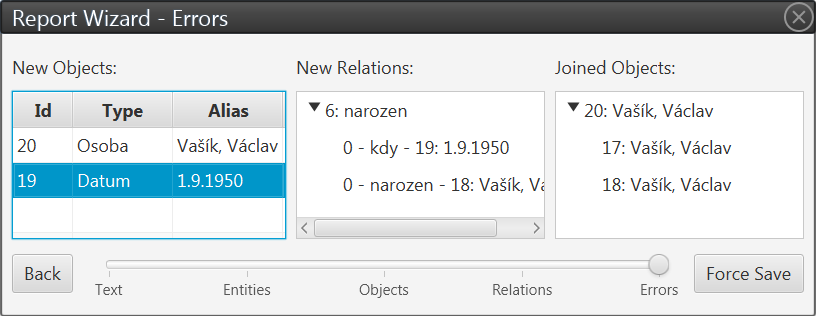
\includegraphics[width=\textwidth]{Images/errors}
        \caption{Errors when saving report.}
        \label{fig:Errors}
\end{figure}

\subsection{Database Exploration}
\label{ssec:ViewDatabase}

Users can use client to view data stored in the database by selecting items
in Dials menu of the main window. Other ways include various context menus
while processing reports etc.

\subsubsection{Browsing Objects}
\label{sssec:ObjectList}

This window contains list of objects matching the filter criteria (alias text,
object type) paginated for more convenient work (see Figure
\ref{fig:ObjectList}. Please note that changing filter criteria must be confirmed by pressing Filter button. Use right mouse button click to open context menu for displaying graph for the selected object (see Section \ref{ssec:Graphs}) or for displaying list of documents containing it (see
Section \ref{sssec:DocumentList}).

\begin{figure}[!htb]
        \centering
        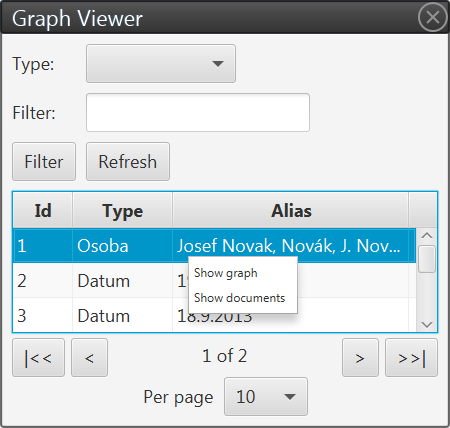
\includegraphics{Images/objectlist}
        \caption{List of objects.}
        \label{fig:ObjectList}
\end{figure}

\subsubsection{Browsing Documents}
\label{sssec:DocumentList}

This window contains list of documents matching filter criteria. Please note
that not all filter controls may be visible at all situations as they are
customized to fit the current context (see Figure \ref{fig:DocumentList}.
Also note that changing filter criteria must be confirmed by pressing Filter
button. Use right mouse button click to open context menu for displaying graph
for the selected document (see Section \ref{ssec:Graphs}) or for displaying the
report itself (see Section \ref{sssec:DocumentView}). Other options include
editing the report or processing it if possible. Inserting new report without processing is done by clicking New document button. Hovering over the row displays full report text.

\begin{figure}[!htb]
        \centering
        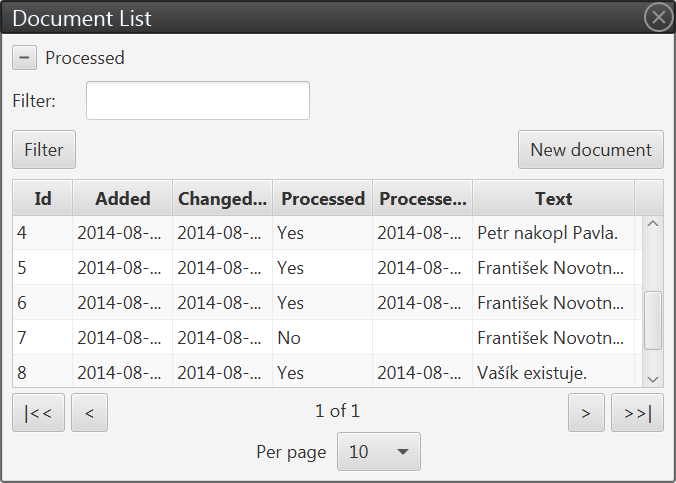
\includegraphics[width=\textwidth]{Images/documentlist}
        \caption{List of documents.}
        \label{fig:DocumentList}
\end{figure}

\subsubsection{Browsing Document}
\label{sssec:DocumentView}

This window displays reports with highlighted objects and relations for easier
orientation (see Figure \ref{fig:DocumentView}). Use right mouse click to open
object context menu to get more information about the selected object. Selecting
relation will highlight its anchor and assigned objects.

\begin{figure}[!htb]
        \centering
        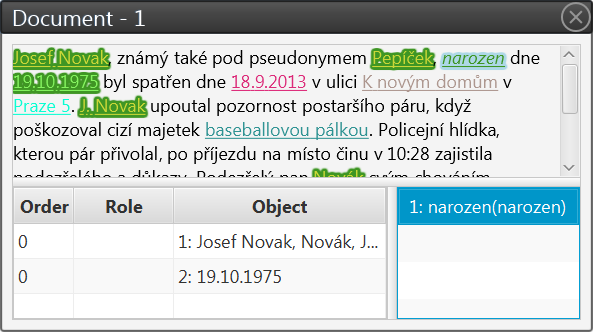
\includegraphics[width=\textwidth]{Images/documentview}
        \caption{Document detail.}
        \label{fig:DocumentView}
\end{figure}

\subsubsection{Browsing Relations}

This window contains list of relations matching the filter criteria (anchor
text, relation type) paginated for more convenient work (see Figure
\ref{fig:RelationList}). Please note that changing filter criteria must be
confirmed by pressing Filter button. Use right mouse button click to open
context menu for displaying graph for the selected relation (see Section
\ref{ssec:Graphs}) or for displaying list of documents containing it (see
Section \ref{sssec:DocumentList}).

\begin{figure}[!htb]
        \centering
        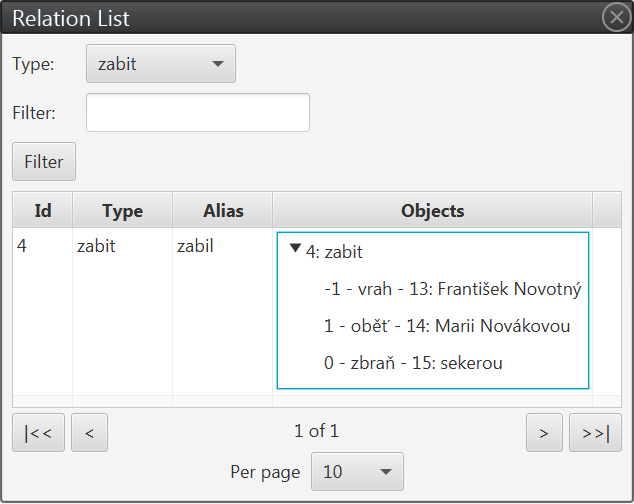
\includegraphics[width=\textwidth]{Images/relationlist}
        \caption{List of relations.}
        \label{fig:RelationList}
\end{figure}

\subsection{Graph Views}
\label{ssec:Graphs}

Graph Windows can be displayed from many places in \textan{} client. Most
common way is right clicking an object/relation/document and selecting Show
graph context menu item.

The graph appearance is drastically effected by Hypergraphs settings (see
Section \ref{sssec:GeneralSettings}).

In the top part of the window (see Figure \ref{fig:Graph}) there is a toolbar
with icons to manipulate the graph.

The first icon represents Transformation and is used to manipulate the graph as a whole, eg. panning or rotating (hold CTRL while left clicking and moving the
mouse). The second icon represents Picking and is used to manipulate subset of
nodes. Hold left mouse button and drag to select multiple nodes and then click
and drag to move them. The third icon centers the view to graph center.
Distance field can be used to change the "radius" around the central node.
Confirm its editing by clicking Go button. Use mousewheel to zoom the graph.

Nodes representing objects can be right clicked to show context menu with
options to display their surroundings or documents. Right clicking edges or
nodes representing the relations shows context menu for centering to objects
assigned to the relation.

On the sides there are lists of object/relation types to display. Unchecking
the type will cause objects/relations of that type to disappear when graph is refreshed by Go button. Clicking the three dots shows or hides the filter
lists.

\begin{figure}[!htb]
        \centering
        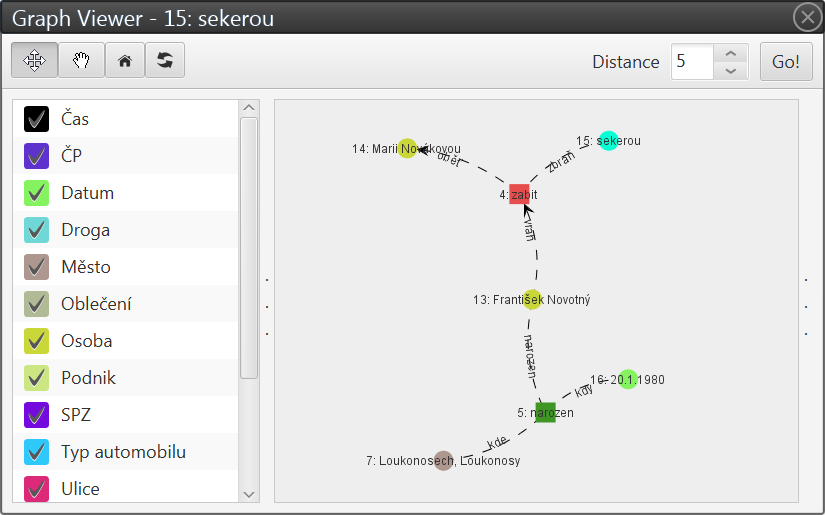
\includegraphics[width=\textwidth]{Images/graph}
        \caption{Graph window.}
        \label{fig:Graph}
\end{figure}

\subsection{Joining Objects}
\label{ssec:JoinObjects}

There can be situations when it is discovered that two objects originally
thought to be independent are in fact one object. For such cases there is Join
Object wizard (see Figure \ref{fig:Join}). For more information about object
lists see Section \ref{sssec:ObjectList}.

\begin{figure}[!htb]
        \centering
        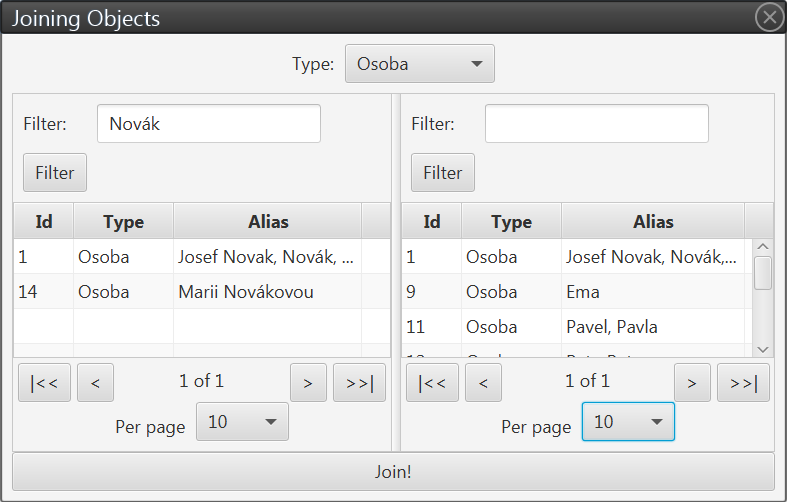
\includegraphics[width=\textwidth]{Images/join}
        \caption{Join Object Wizard.}
        \label{fig:Join}
\end{figure}

The objects to merge must have common type. Select one object in left object
list and the other one in right object list. The button Join will start the
joining itself.

\subsection{Path Wizard}
This wizard displays window similar to Joining Objects. Select two objects
for which you want to try to find path of relations and objects connecting them
(see Figure \ref{fig:Path}). You can also specify the maximal length of the
path. The greater the maximal distance, the longer can take to find the path.
The system looks only for the shortest route. If such path is found, the graph
displaying it is shown (see Figure \ref{fig:PathGraph}).

\begin{figure}[!htb]
        \centering
        
\includegraphics[width=\textwidth]{Images/path}
        \caption{Path Wizard.}
        \label{fig:Path}
\end{figure}

\begin{figure}[!htb]
        \centering
        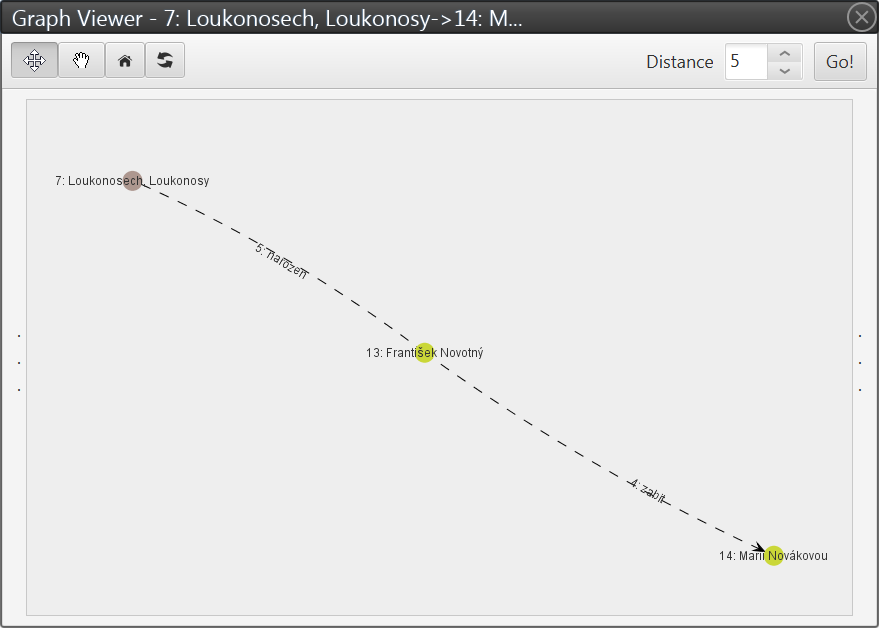
\includegraphics[width=\textwidth]{Images/pathgraph}
        \caption{Graph displaying the path between objects.}
        \label{fig:PathGraph}
\end{figure}
